\chapter{Background and Related Work}

\label{ch:background} 
\label{sec:background}

%A literature and technology review, leading up to the problem that is tackled—you should show a knowledge and awareness of the relevant literature and/or technologies. You shouldn't just give a descriptive list of other work: you should organise the work that you review in an appropriate scheme, show connections and contrasts between the work, point out the strengths and weaknesses of existing work, and where appropriate clearly identify what the current state-of-the-art approaches are to the problem.

Explaining what your project does that is new or is better than existing work in the same field.



Talk through different models and their strengths/weaknesses:
\section{Early Chatbots}
\label{sec:background_early_chatbots}

The earliest chatbots used rule-based technology to respond to textual inputs. One of the earliest chatbots was Eliza, created in 1966 by researchers at MIT to pass the Turing Test \citep{zemvcik2019}. It used pattern matching to be able to construct human-like replies \citep{Luka}. However, the responses were often formulaic and predictable. Such systems were limited by the complexity of natural language, as it is highly difficult and inefficient to generate rules to handle every possible query. A number of adaptations have been made since these early frameworks, which are outlined below.

%The development of \acrfull{ai} and \acrfull{nlp} meant that chatbots began to learn from data and

\section{\acrlong{ann}s}
\label{sec:background_anns}

\acrlong{ann}s (\acrshort{ann}) are part of a branch of machine learning called deep learning, with machine learning itself being a branch of \acrlong{ai}. \acrshort{ann}s seek to provide solutions to a wide range of classification, pattern recognition and prediction problems, and are used extensively in image recognition and \acrfull{nlp} tasks \citep{Abiodun}. Inspired by the human brain, they are analogous to the nervous system; they take an input and, using a set of complex neurons, seek to identify an output response \citep{Bishop}. They do this by learning from examples, in a similar way to humans. For example, \acrshort{ann}s can be used to predict whether an image contains a pizza or a football.

\subsection{Structure}
\label{sec:background_anns_structure}
Neural networks take a series of inputs (via the input layer) and seek to predict the output (via the output layer). In order to do this, they often contain a number of `fully connected' hidden layers of a pre-determined size that consist of neurons and nodes which themselves contain weights and biases. The size of the input layer is determined by the attributes/information that the model has available to it, and the size of output layer is determined by the classification/prediction problem. 

\begin{figure}[h]
    \centering
    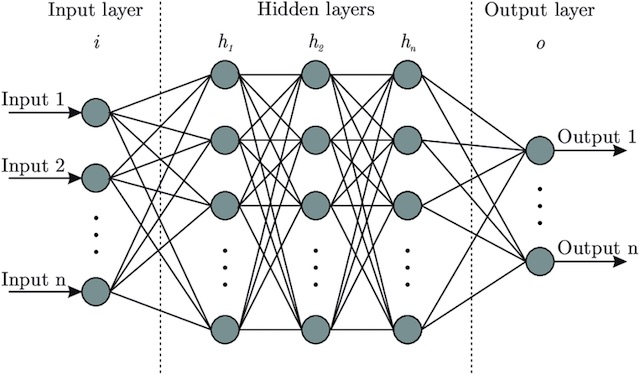
\includegraphics[height=5.5cm] {Paper/images/neural_network_structure.jpeg} % ,trim={0 0 0 0cm},clip
    \caption{Typical Neural Network Structure \citep{Shukla}}
    \label{fig:neural_network_structure}
\end{figure}

This structure is shown in Figure \ref{fig:neural_network_structure}, where each grey circle denotes a node, and each interconnecting line denotes a weight between two nodes. As can be seen, each node is connected to every node in the next layer (in a fully connected layer), and the value of each node in the next layer is a weighted sum of the values of the nodes in the previous layer and their corresponding weights (and sometimes a bias term) \citep{Bishop}. The weights therefore determine how much information is passed on to each node in the next layer. The weights are analogous to the strength of connection of biological neurons, and the bias is analogous to the firing threshold.

\subsection{Activation Functions}
\label{sec:background_anns_activation_functions}

The value in each node is of a neural network is typically transformed by an activation function, often Sigmoid or \acrfull{relu}. The former ensures that the values are non-linearly scaled to be between 0 and 1 using $f(x) = \frac{1}{1+e^{-x}}$, whereas the latter truncates values that were below 0 to be 0 using $f(x) = max(0, x)$. Therefore the range of a sigmoid activation function is $(0, 1)$ and the range of a \acrshort{relu} activation function is $[0, \infty]$. These activation functions, along with some other common ones, are shown in Figure \ref{fig:activation_functions}.

\begin{figure}[h]
\centering
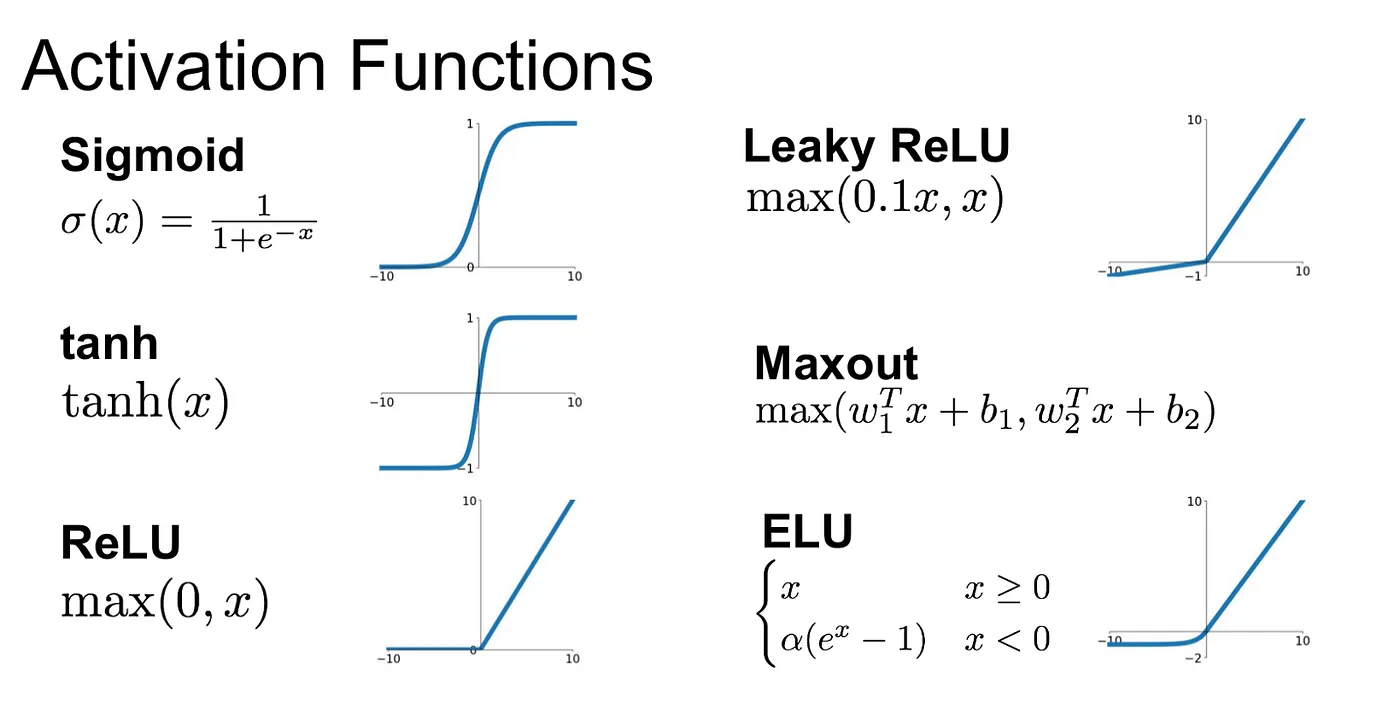
\includegraphics[height=5.5cm,trim={0 0 0 3.5cm},clip]{Paper/images/activation_functions.png}
\caption{Activation Functions used in Neural Networks \citep{Udofia}}
\label{fig:activation_functions}
\end{figure}

This process is continued for each of the (fully connected) hidden layers, until the network has calculated the values for each of the nodes in the output layer. This will typically be a proportion which, in the case of next sentence prediction, denotes the likelihood of that specific word being the next word in the sentence.

\subsection{Learning}
\label{sec:background_anns_learning}
The learning in neural networks occurs in training the weights that connect each of the nodes. \acrlong{ann}s use a technique known as forward propagation to calculate the predicted output from a given input. Initially, the weights in the network are randomly assigned \citep{Bishop}, meaning that the model has essentially no prior predictive power. For each example data point the network calculates the values for each of the nodes in the output layer; these denote "the probability that the given input fits into each of the pre-set categories" \citep{Yathish}. This process is repeated for each of the training examples, and is known as Forward Propagation. 

The predicted values are subsequently compared against the expected (true) value, and the model and computes the error (the difference between the predicted and true values). This error is fed into a loss function, which a measure of the inaccuracy of the model; the aim is to minimise the loss function. For most classification problems, a Cross-entropy (log loss) function is used.

Once the value for the loss function has been calculated, the model then seeks to update weights and biases in each layer, using a process called  Back-propagation \citep{Rumelhart}. This process begins by computing $\partial E/ \partial y$ for each of the output units. By using the chain rule, we can expand this



\section{\acrlong{rnn}s}
\label{sec:background_rnns}
\acrlong{rnn}s are a form of neural network used for sequential data. They take each element of the sequence one at a time and use the current and previous values to predict future ones. They can crudely be thought of as ``very deep feedforward networks in which all the layers share the same weights'' \citep{Yann}. However, when backpropagation is used to train the network, problems are often encountered.

A common problem with training neural networks is the vanishing/exploding gradient problem \citep{hochreiter1997long}. This can occur in deep neural networks but is particularly common in \acrshort{rnn}s, as the same weights are used in each iteration. The exploding gradient problem is where the model weights become exponentially large, which causes the model weights to become NAN. Alternatively, because of the recurrent structure of the model, there can be a tendency for model weights to `vanish' and tend to 0. This causes the model to have short-term memory because it fails to capture long-term dependencies \citep{chung2014empirical}. In addition to this, in both cases, the loss function is not minimised because the weights cause the loss function to either overshoot or never reach the global/local minimum.

\subsection{\acrlong{lstm} Cells}
\label{sec:background_lstms}
\acrshort{lstm} networks are a type of \acrlong{rnn} which were developed by \citet{hochreiter1997long} in order to overcome the vanishing/exploding gradient problem. They use sigmoid and tanh activation functions as part of 3 `gates' (input gate, forget gate, and output gate) to determine how much of the long-term memory is maintained and to update both the long-term and short-term memory in each cell. They overcome the vanishing and exploding gradient problem because they control how much the gradient vanishes using the `forget gate' \citep{Gers}.

\subsection{\acrlong{gru}s}
\label{sec:background_grus}
Another similar model to \acrshort{lstm}s is the \acrfull {gru}, with an architecture based on just two gates (reset gate and update gate). It was developed in 2014 by \citet{cho2014learning} and provides a simpler architecture than the \acrshort{lstm} model. The flow of information is held using a `hidden state' and the two gates determine how much information it remembers or forgets.

The update gate determines how much of the memory it retains, and the reset gate determines how much of the memory it forgets.

\acrlong{lstm} cells and \acrlong{gru}s often perform similarly effectively. However, it has been noted in the literature that \acrshort{gru}s generally outperform LSTM networks on sequences that are short and less complex, whereas \acrshort{lstm} models are typically favoured for longer and more complex sequences \citep{cahuantzi2023comparison}. This is often attributed to the \acrshort{lstm} model's ability to better capture long-term dependencies in sequences, which often means it is preferred for language modelling \citep{Irie2016}. However, both models can only capture forward dependencies, due to their sequential nature. For example, with the sentence `Joel read a book about a bass that was owned by a fisherman', using only the first 7 words, you would not know whether the word `bass' refers to the fish or the instrument. It is only with the latter parts of the sequence that you can determine the context and therefore the bass was owned by the fisherman and not the musician. Therefore, models which only capture forward dependencies will miss any potential inference based on future words. 

\subsection{Bidirectional \acrlong{rnn}s}
\label{sec:background_bidirectional_rnns}
To overcome this limitation, Bidirectional \acrshort{rnn}s were developed by \citet{Schuster} and are a combination of two \acrshort{rnn}s (Section \ref{sec:background_rnns}). One processes information in the usual chronological manner, with a second processing it in reverse time order. The model is trained simultaneously on both of these and seeks to minimise the loss function for both time directions concurrently. This allows the model to capture the future context in sequences, which is particularly important in \acrshort{nlp} implementations because the context of words is typically derived from future words.

All of the above models (\acrshort{rnn}s, \acrshort{lstm}s, and \acrshort{gru}s require sentences to be processed sequentially, and so can take a very long time to train). We will now explore 2 alternative models which seek to solve this.

\section{\acrlong{cnn}s}
\label{sec:background_cnns}


\section{Transformers}
\label{sec:background_transformers}

\subsection{Bidirectional \acrshort{rnn}s}
\subsection{Embeddings}
Bengio et. al., 2003 talks about how integer IDs are inferior to vector representations of words, as vector representations enable similar words to be `close' together/have some similarity mathematically.

word embedding = feature vector representation of a word. But word2Vec is bad. Word2Vec generates a vector representation of words (king-woman+man=?) but it doesn't provide contextualisation. This means that you can't distinguish between a `fun fair' and a `process being fair'. Therefore it is essential to generate contextualised embeddings/representations. (this uses its placement within a sentence using the sin/cos functions? What about the sentence placement - which sentence it is?) Therefore we can have similar representations of fair/unbiased and fair/carnival.

Use BERT's pre-training (Self-supervison) to generate contextual encodings for words? And then use fine-tuning/feature-based approach for use with another model.






% ----------------------------------------------------------------------------------------------------------------------
History of improvements: 
ELMo - 2 bi-directional RNNs. But it is an LSTM and so doesn't make use of GPUs and so it very slow.
Transformer Neural Networks - encoders and decoders
OpenAI's GPT uses stacked decoders
BERT uses stacked encoders - masked language model and next sentence prediction.
BART uses both

RNNs have historically been the industry standard, due to the sequential structure of language, but they are slow to train (due to sequential processing of each token) \citep{vaswani2017attention}, especially when there are long strings to process, and can have convergence issues due to vanishing/exploding gradients \citep{Lipton}.

% From file:///C:/Users/point/Downloads/QA-CEP-2020.pdf:
• Much early NLP work attempted reading comprehension
– Schank, Abelson, Lehnert et al. c. 1977 – “Yale A.I. Project”
• Revived by Lynette Hirschman in 1999:
– Could NLP systems answer human reading comprehension questions for 
3rd to 6th graders? Simple methods attempted.
• Revived again by Chris Burges in 2013 with MCTest
– Again answering questions over simple story texts
• Floodgates opened in 2015/16 with the production of large datasets which 
permit supervised neural systems to be built
– Hermann et al. (NIPS 2015) DeepMind CNN/DM dataset
– Rajpurkar et al. (EMNLP 2016) SQuAD
– MS MARCO, TriviaQA, RACE, NewsQA, NarrativeQA, HotpotQA
%

Not simply question answering (copying and pasting an answer), but generative question answering (generate text/summarise text to provide an answer)

Use hugging face library - many pre-trained models

IBM Watson was famously developed to compete on the quiz show Jeproady! and beat the then-champions to win 1st prize https://web.archive.org/web/20130616092431/http://www.jeopardy.com/news/watson1x7ap4.php


 

Complexity of human language means that a `bag-of-words' approach can only have limited success in understanding human language.

Context.

neural networks and convolutional neural networks have been used to improve chatbot performance.

question answering chatbots have gone from ***? question answering to generative question answering, where they use probabilities to generate text. By learning the patterns and semantics of language, it can generate human-like responses. Initially, Markov Chains were used to generate the most probable characters or words in the output (e.g. HeX) \citep{Luka, Ahmad}. 

BERT (Devlin et al., 2019), T5 (Raffel et al., 2019), and GPT-3 (Brown et al., 2020)

A CNN uses convolutions for feature extraction and a fully connected neural network for the classification \citep{Budiharto}. "RNN excels in the sequence of data, like time series or sentence, but RNN has a problem in long-term dependency (the capability to remember information for a long period of time). Long Short Term Memory (LSTM) and Gated Recurrent Unit (GRU) are the improvements of RNN. LSTM composed of a cell, an input gate, an output gate and a forget gate. Memory cells and gate units in LSTM learns to protect the constant error flow within the memory cell from perturbation by irrelevant inputs [18]. GRU consists of two gates, Reset Gate and Update Gate [19]. Te Update Gate is the merging of Forget Gate and Input Gate in LSTM."

Deep learning is a subfield of Machine Learning, with vast applications, particularly within computer vision and \acrshort{nlp}

"A comparative study of CNN and RNN for NLP explored by Yin et  al. [http://arxiv.org/abs/1702.01923] shows that RNN performs better than CNN in most of the NLP tasks" https://journalofbigdata.springeropen.com/articles/10.1186/s40537-020-00341-6


Squad \acrshort{squad} data reference: http://arxiv.org/abs/1606.05250, and for squad 2.0: http://arxiv.org/abs/1806.03822

By using a BiDAF combined with RNN and CNN encoders, \citep{Budiharto} found that an RNN-based encoder had a higher F1-score than a CNN-based encoder when using the \acrshort{squad} dataset.

Translation, sentiment analysis and emotion detection \citep{Hirschberg}



From ChatGPT:
1. Rule-Based Chatbots: Limited, inflexible, and prescriptive responses.

2. Natural Language Processing (NLP): Supports the understanding and interpretation of language

3. Machine Learning (ML): Learn from user interactions and improve responses over time by identifying patterns in user input and tailor their responses accordingly.

4. Artificial Inteligence (AI): Specifically deep learning, which enabled the understanding of context and means chatbots can provide personalized responses.